\begin{figure*}
\begin{subfigure}{0.195\textwidth}
\centering
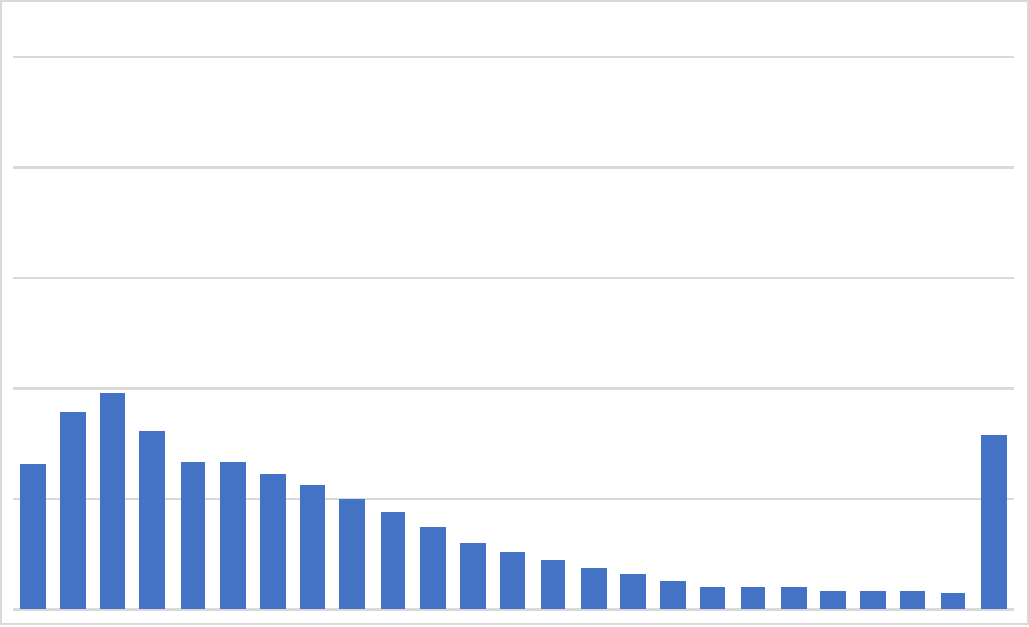
\includegraphics[width=0.9\linewidth]{results/cloverleaf3d/eul_1/Eul1_AvgL2.pdf}
\vspace{-2mm}
\caption{Eul 20 Avg$_{L2}$ L2 }
\end{subfigure}
\begin{subfigure}{0.195\textwidth}
\centering
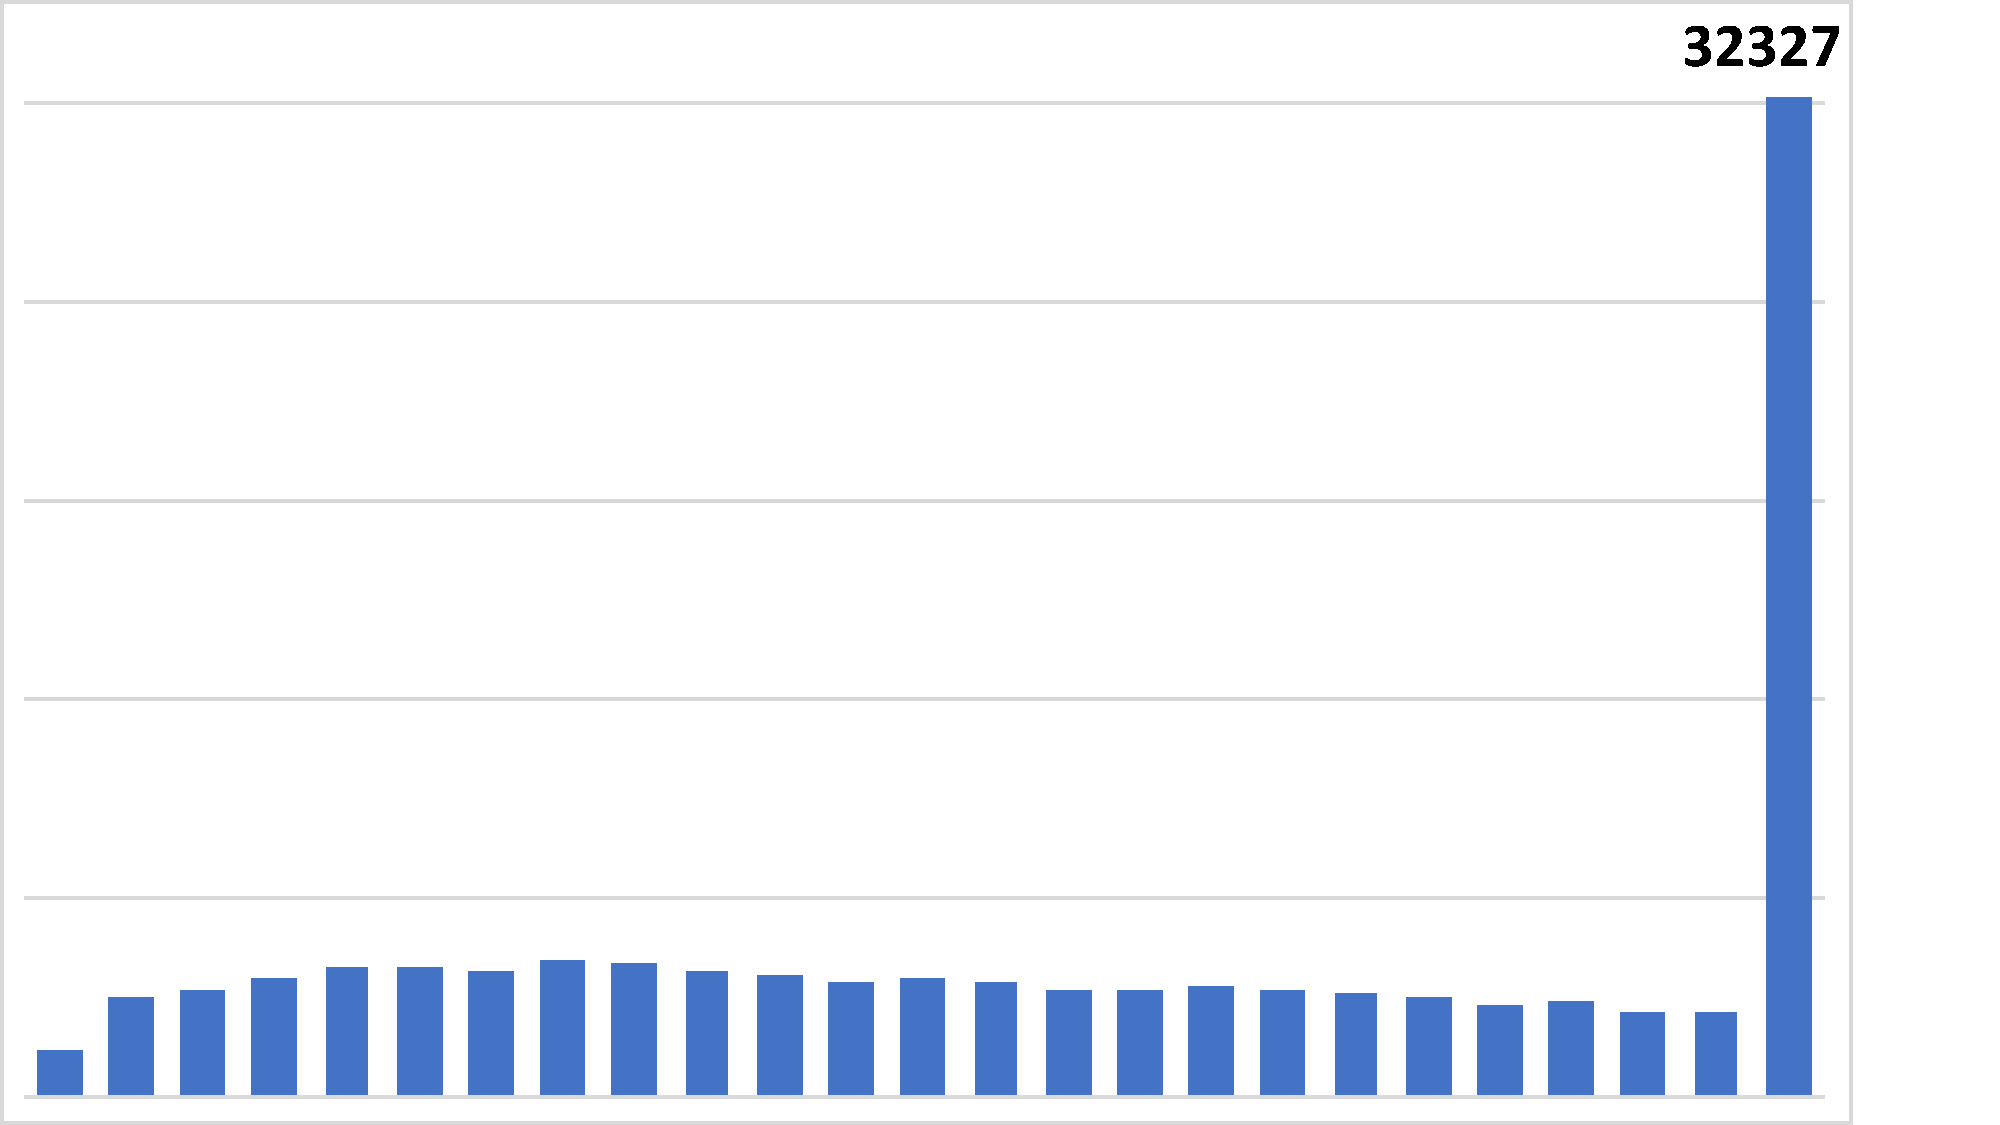
\includegraphics[width=0.95\linewidth]{results/cloverleaf3d/eul_2/Eul2_AvgL2.pdf}
\vspace{-2mm}
\caption{Eul 40 Avg$_{L2}$ L2 }
\end{subfigure}
\begin{subfigure}{0.195\textwidth}
\centering
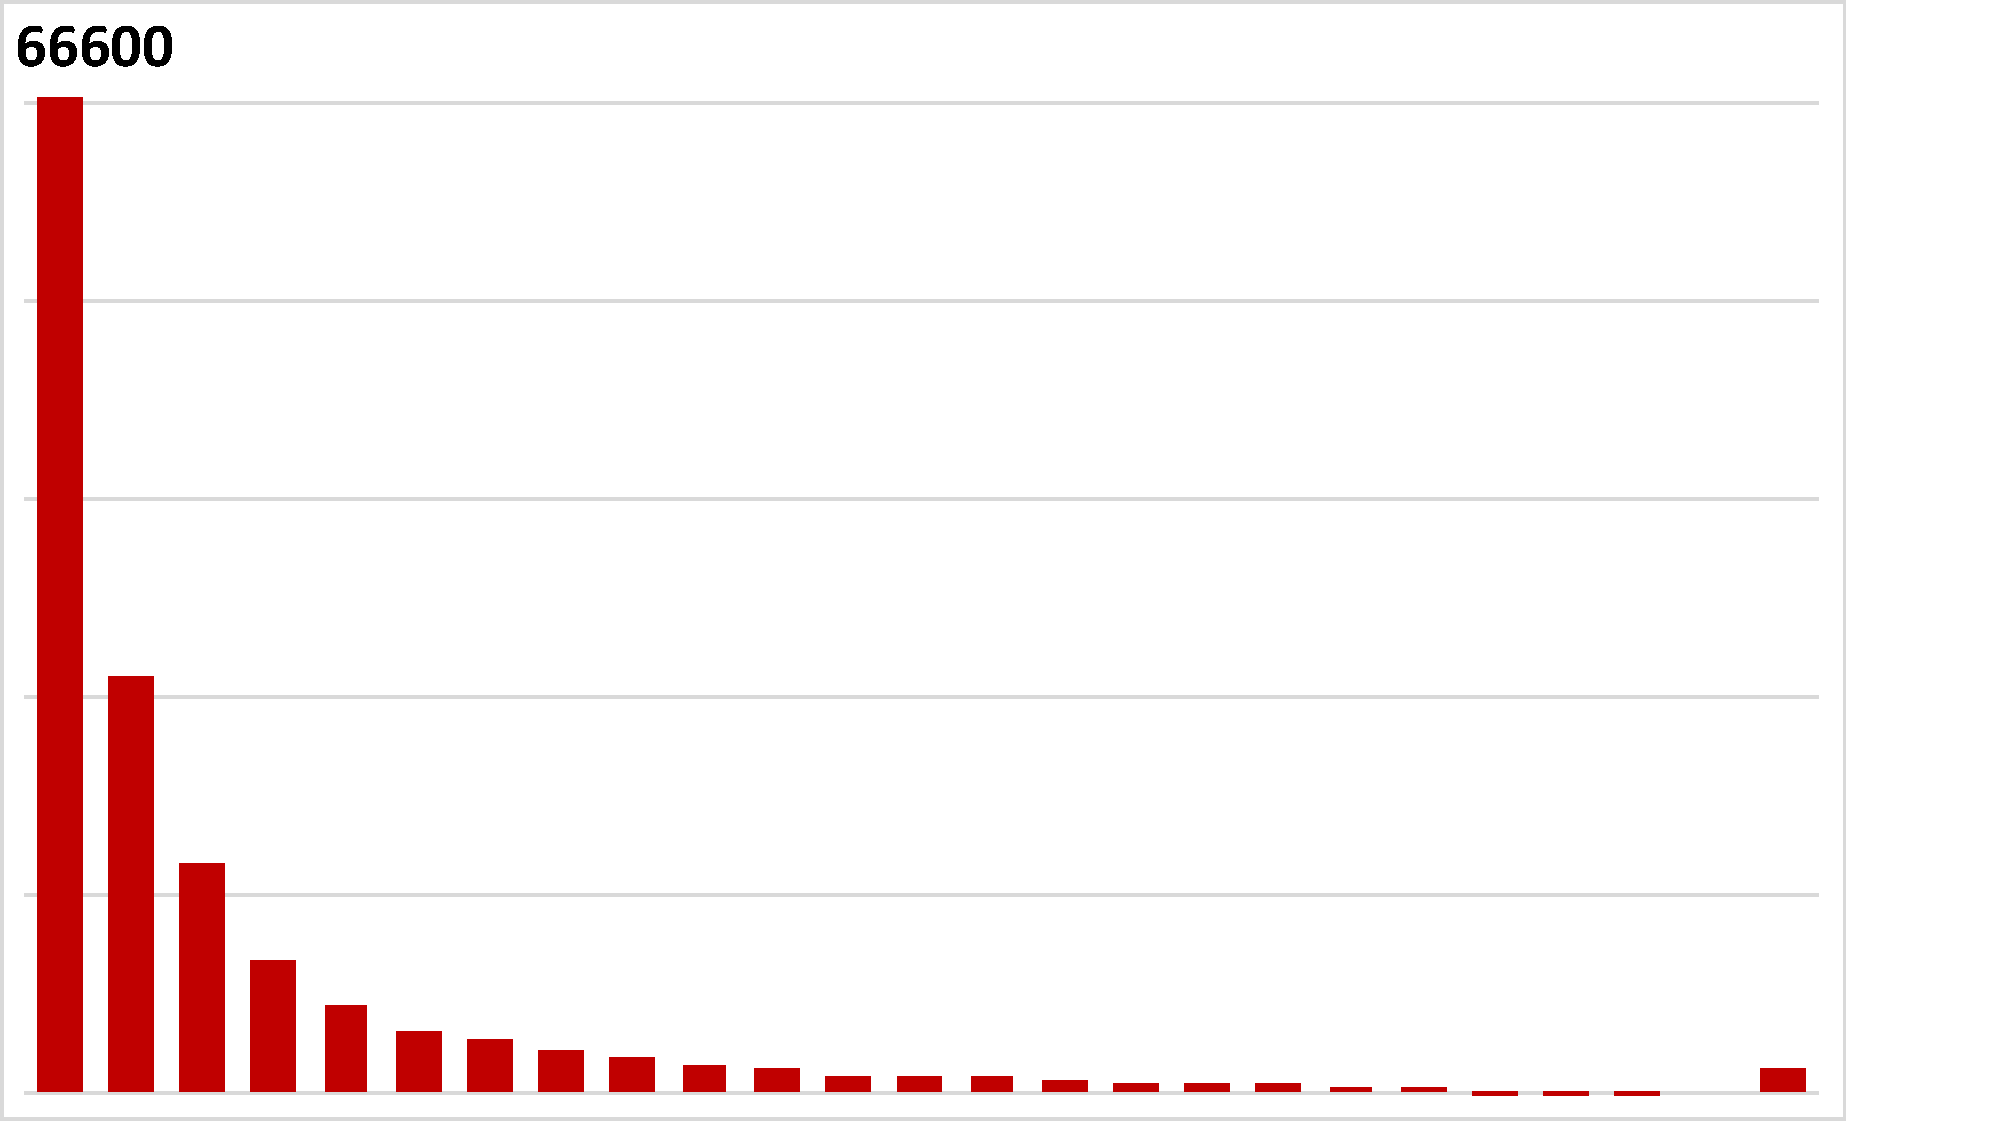
\includegraphics[width=0.9\linewidth, trim={0cm 0cm 2.5cm 0cm}, clip]{results/cloverleaf3d/lag_4/Lag4_AvgL2.pdf}
\vspace{-2mm}
\caption{Lag 40 1:8 Avg$_{L2}$ }
\end{subfigure}
\begin{subfigure}{0.195\textwidth}
\centering
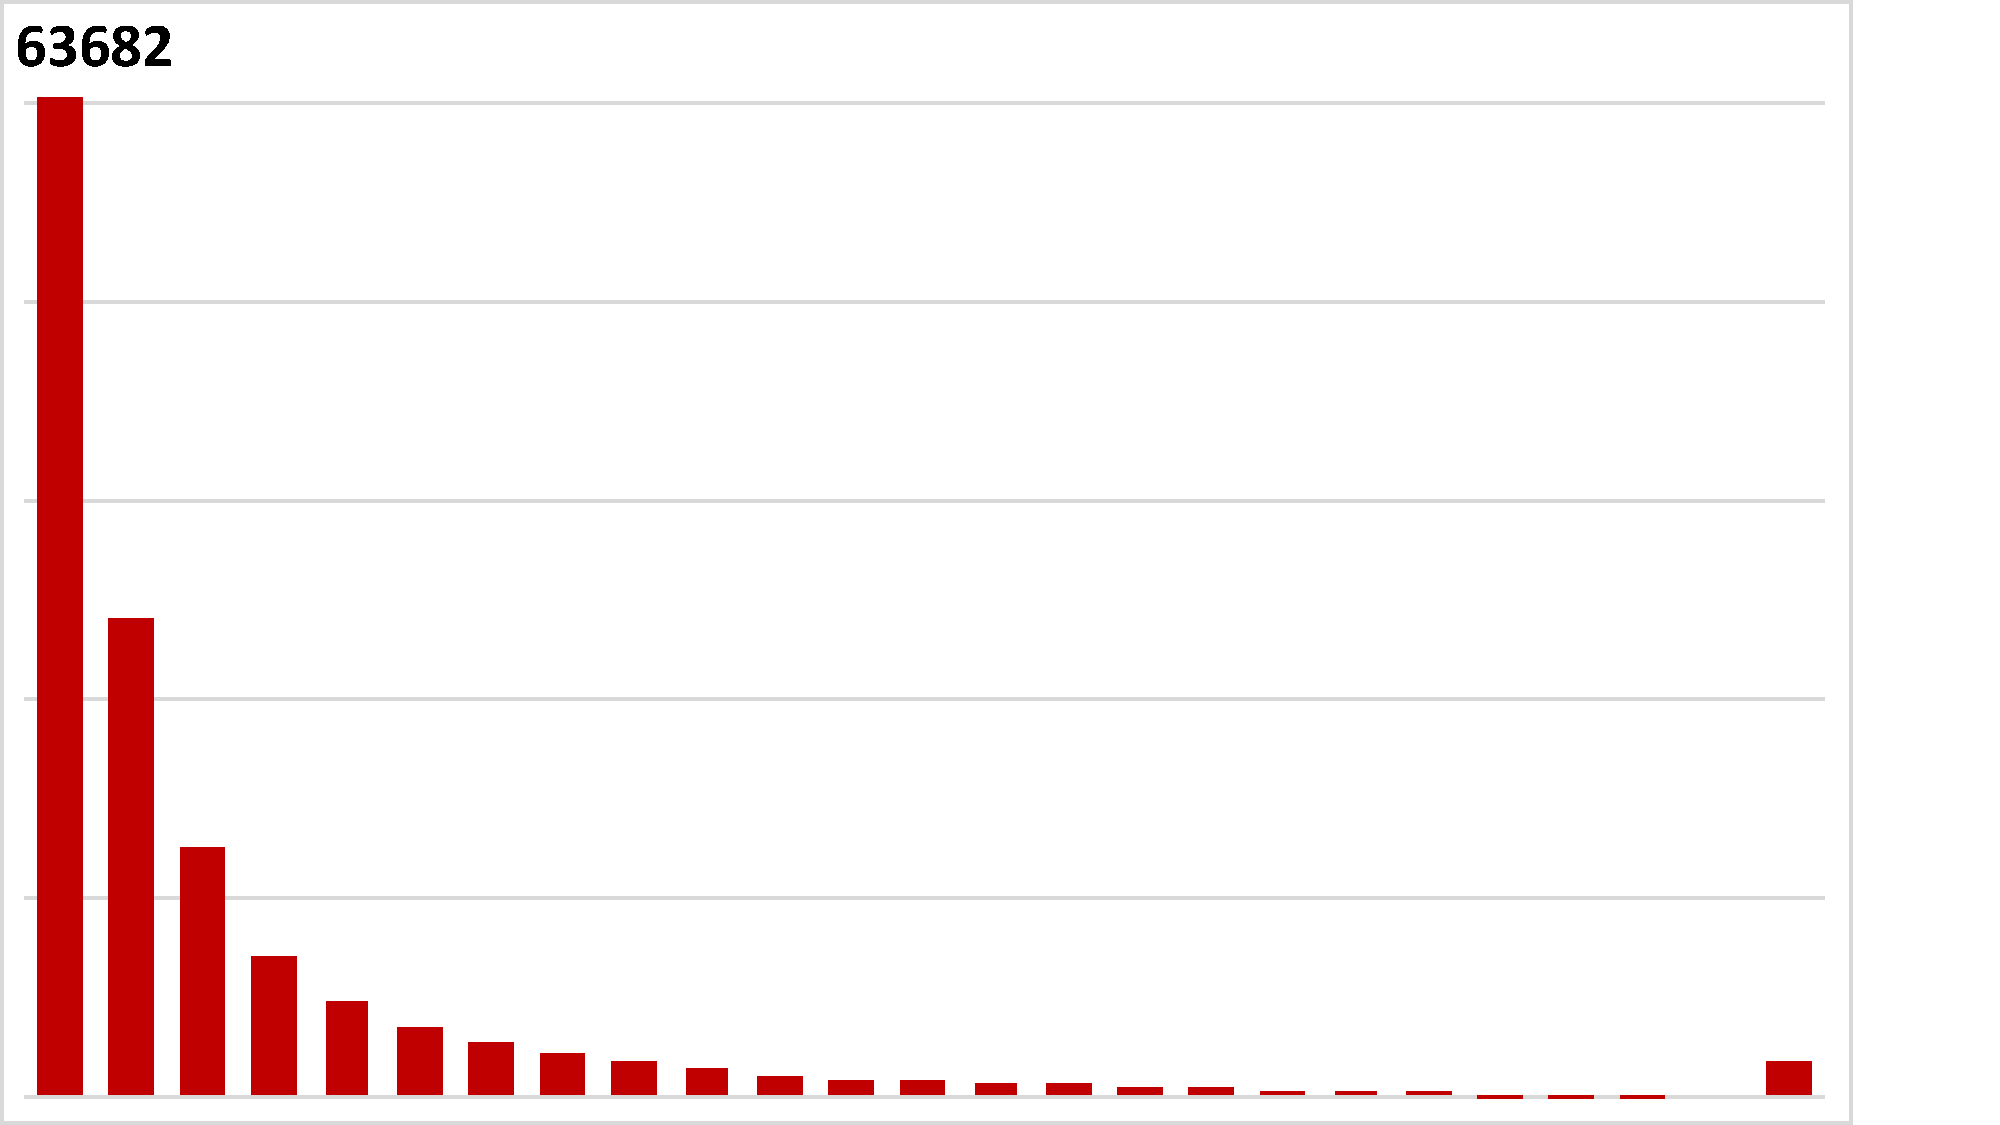
\includegraphics[width=0.9\linewidth, trim={0cm 0cm 2.5cm 0cm}, clip]{results/cloverleaf3d/lag_5/Lag5_AvgL2.pdf}
\vspace{-2mm}
\caption{Lag 40 1:27 Avg$_{L2}$ }
\end{subfigure}
\begin{subfigure}{0.195\textwidth}
\centering
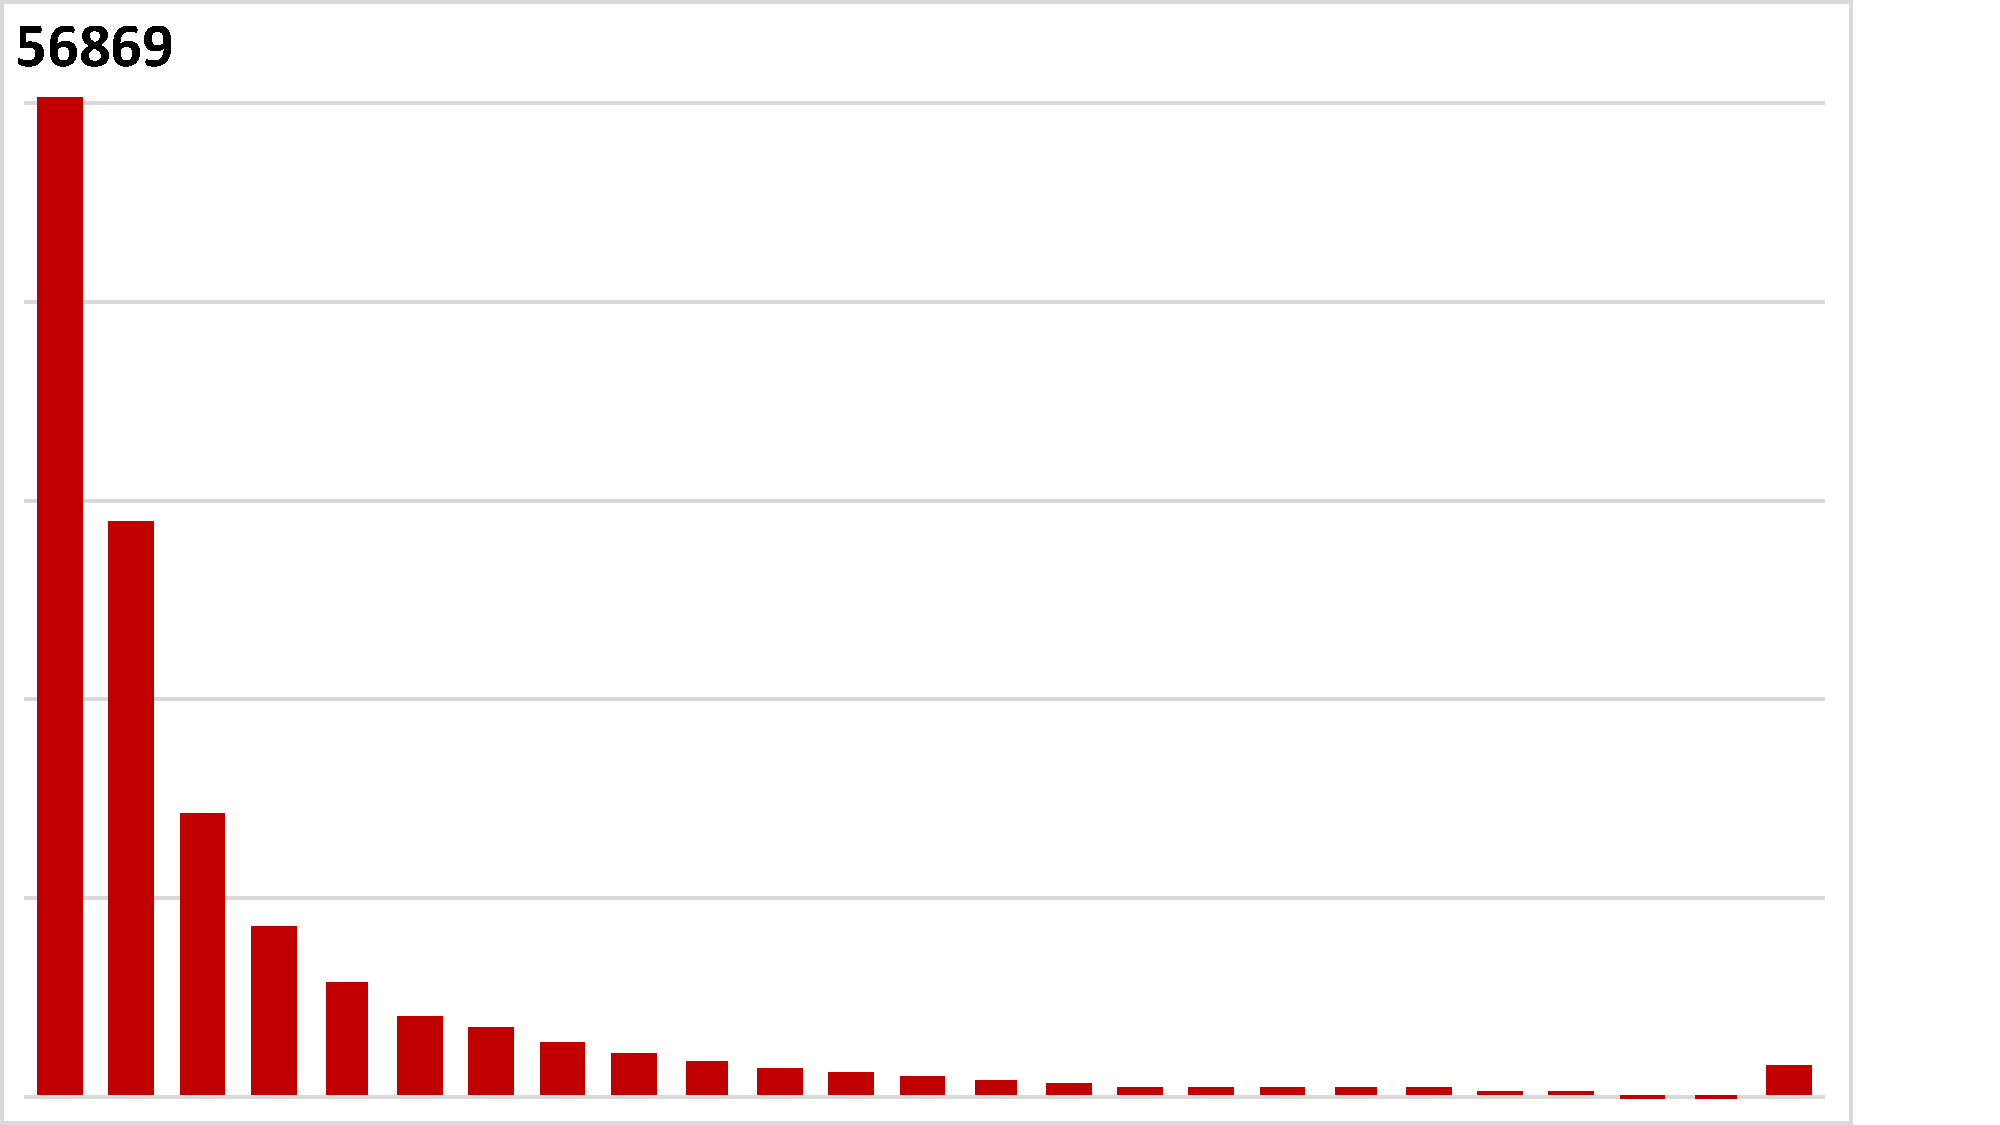
\includegraphics[width=0.9\linewidth, trim={0cm 0cm 2.5cm 0cm}, clip]{results/cloverleaf3d/lag_6/Lag6_AvgL2.pdf}
\vspace{-2mm}
\caption{Lag 40 1:64 Avg$_{L2}$ }
\end{subfigure}
\begin{subfigure}{0.195\textwidth}
\centering
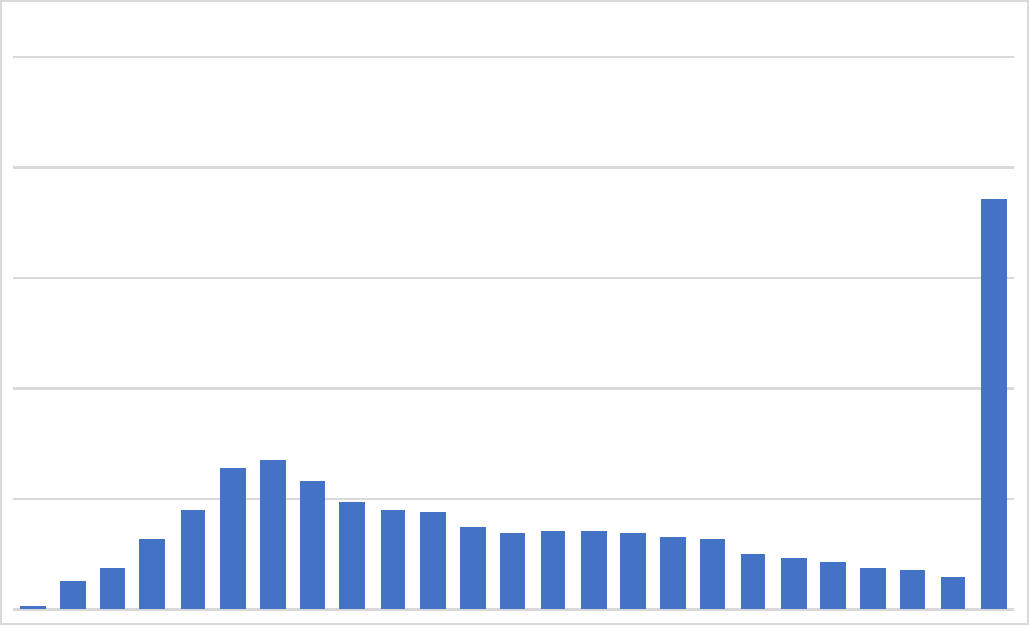
\includegraphics[width=0.9\linewidth]{results/cloverleaf3d/eul_1/Eul1_Max.pdf}
\vspace{-2mm}
\caption{Eul 20 Max$_{L2}$ }
\end{subfigure}
\begin{subfigure}{0.195\textwidth}
\centering
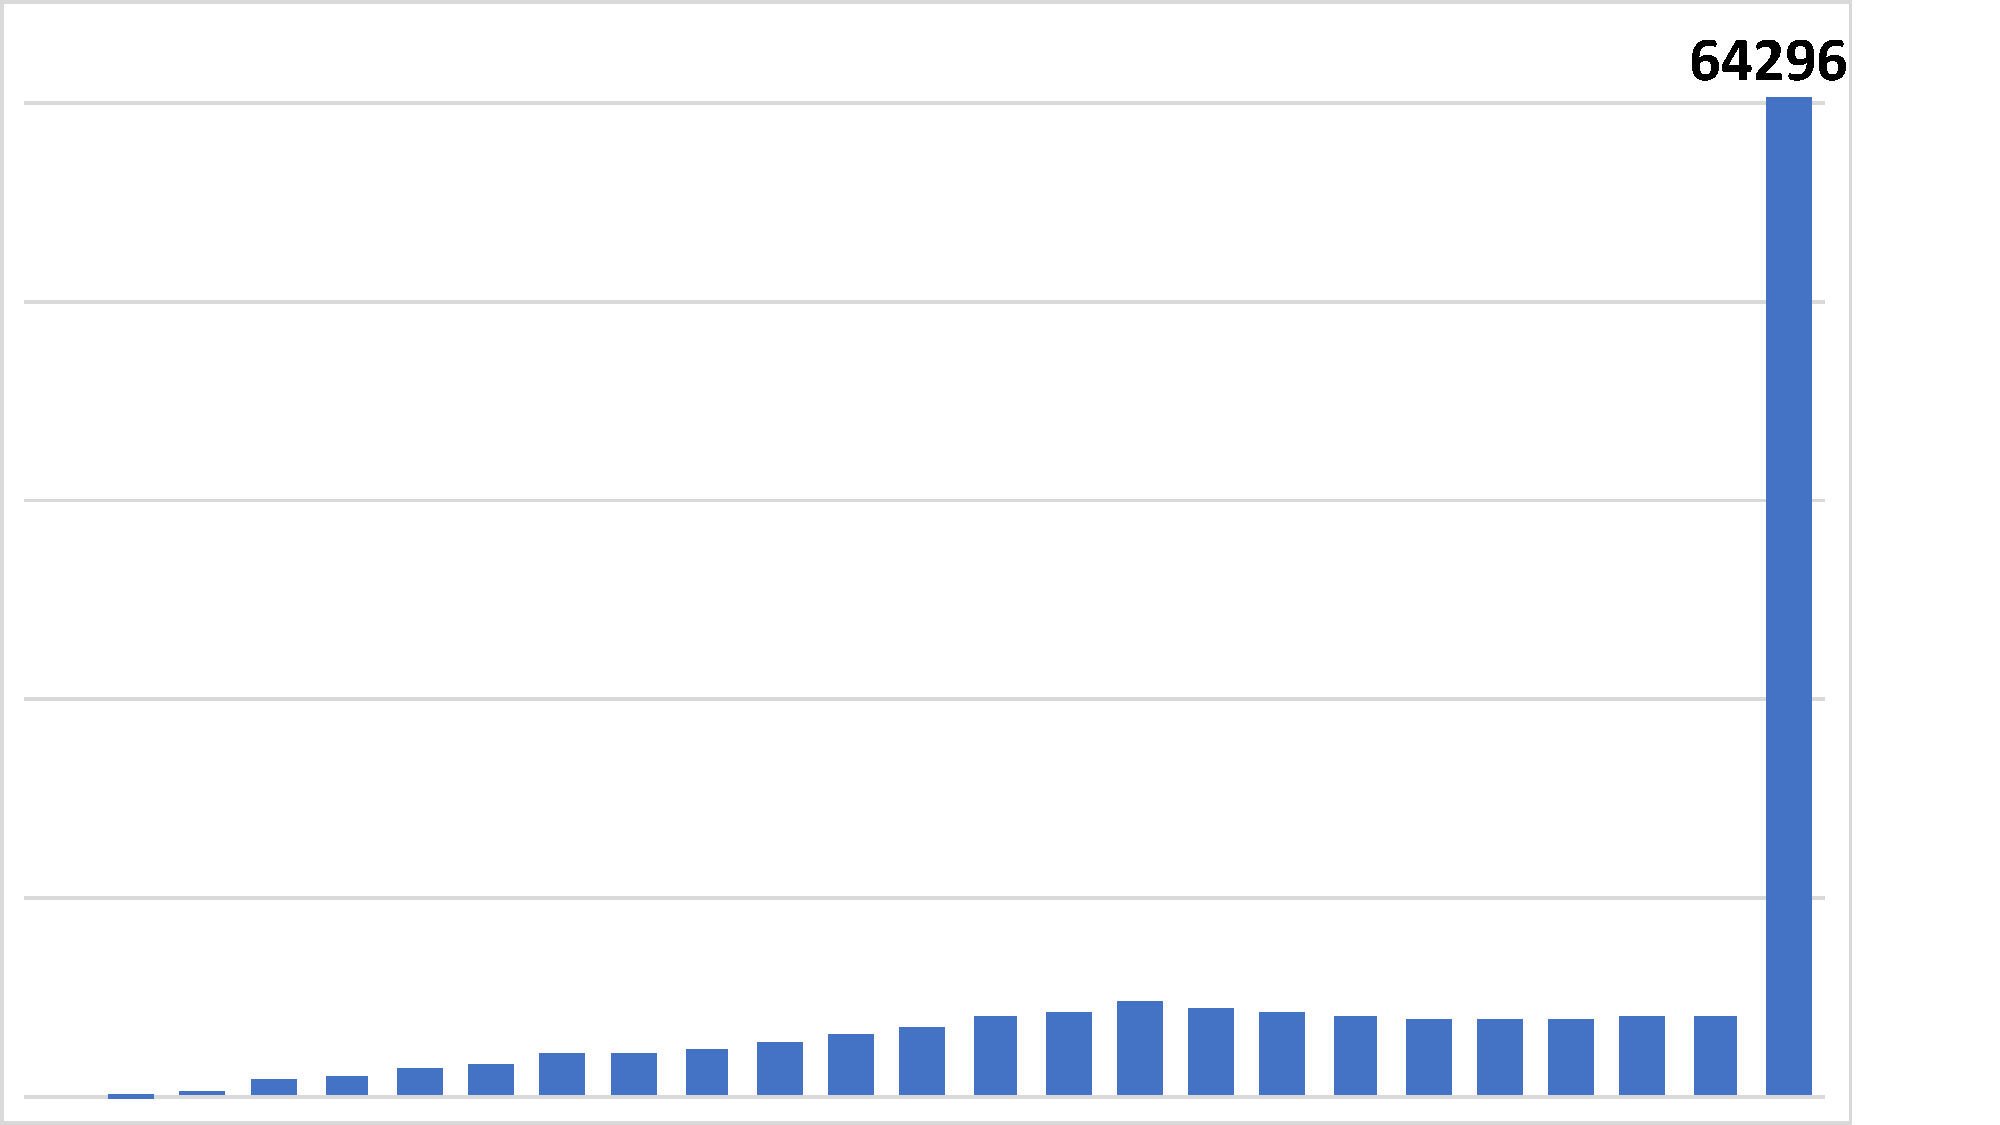
\includegraphics[width=0.95\linewidth]{results/cloverleaf3d/eul_2/Eul2_Max.pdf}
\vspace{-2mm}
\caption{Eul 40 Max$_{L2}$ }
\end{subfigure}
\hspace{0.2mm}
\begin{subfigure}{0.195\textwidth}
\centering
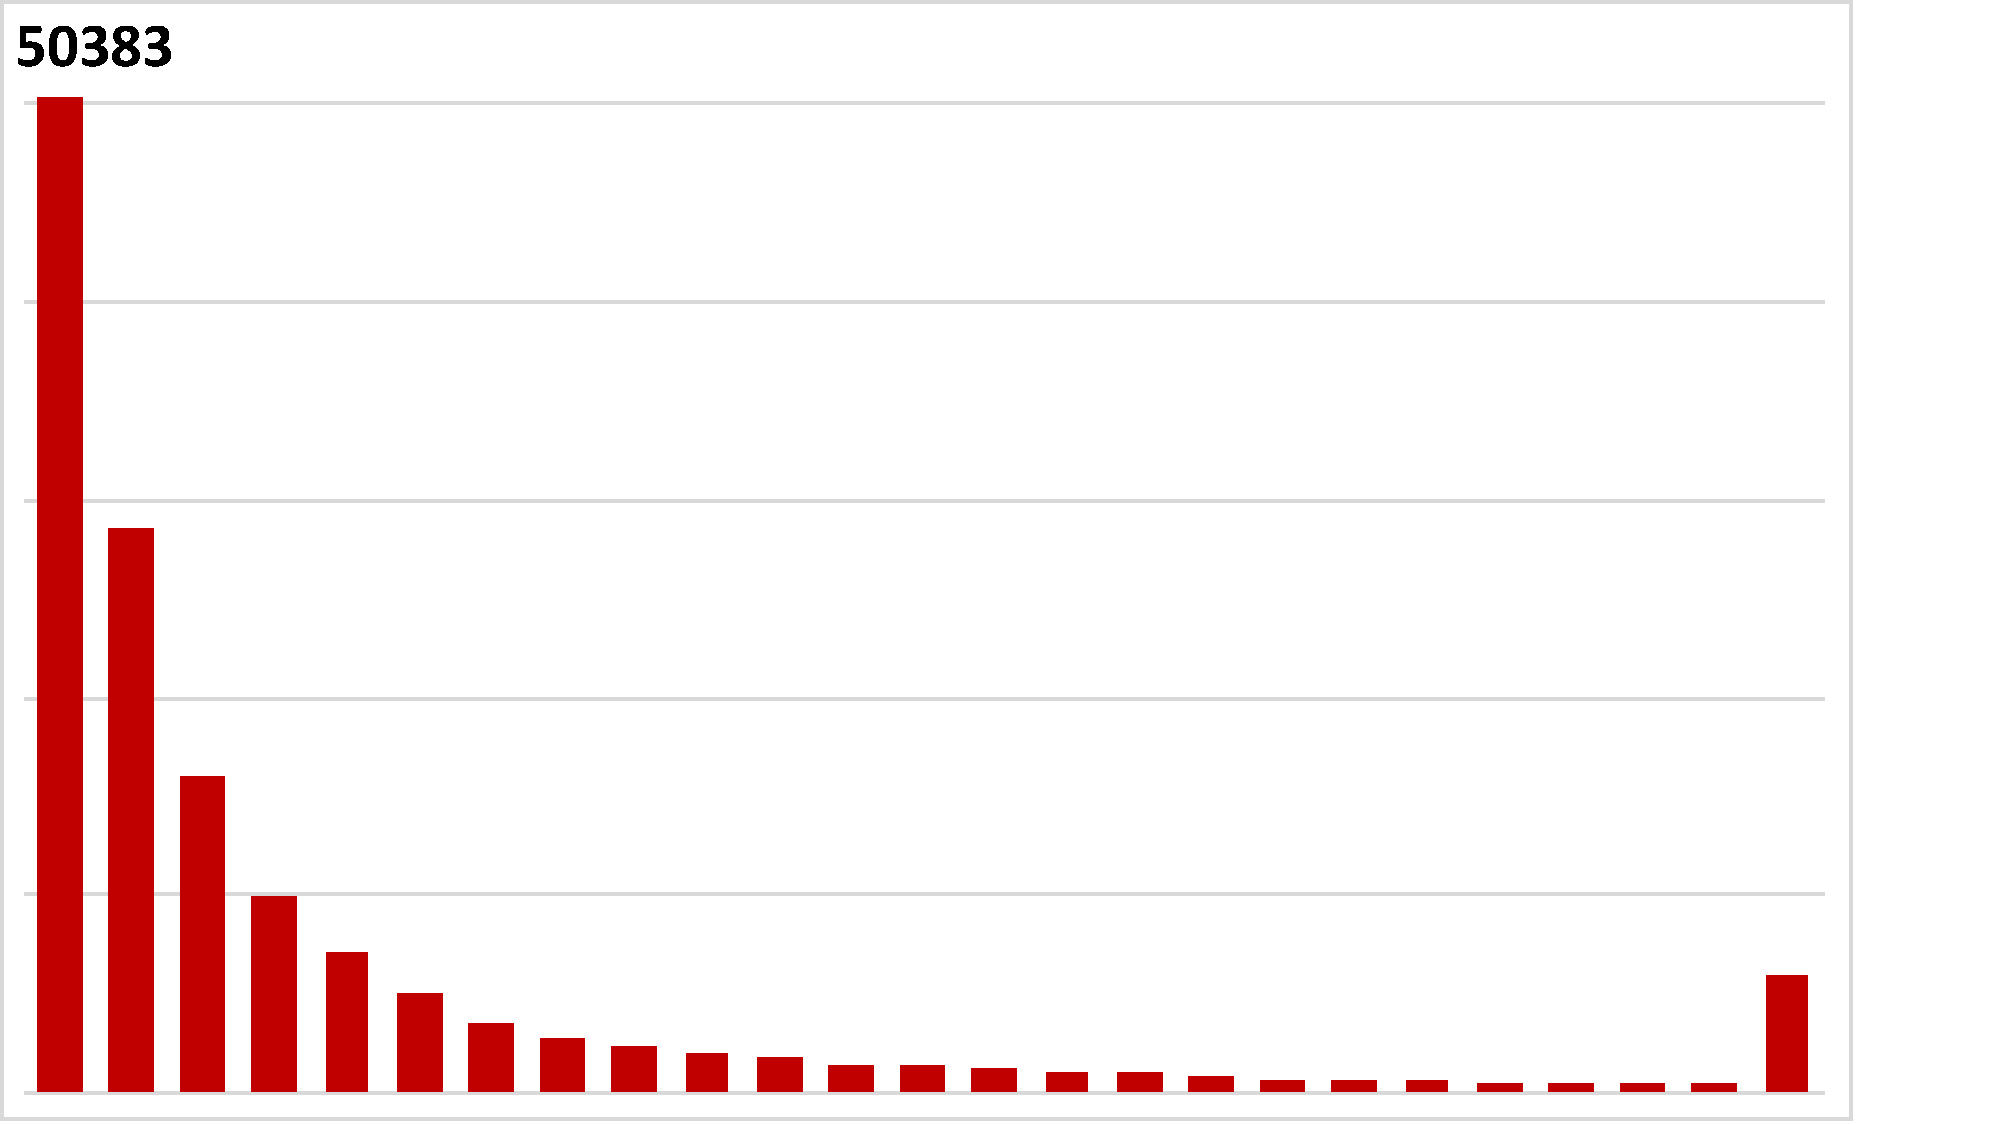
\includegraphics[width=0.9\linewidth, trim={0cm 0cm 2.5cm 0cm}, clip]{results/cloverleaf3d/lag_4/Lag4_Max.pdf}
\vspace{-2mm}
\caption{Lag 40 1:8 Max$_{L2}$ }
\end{subfigure}
\begin{subfigure}{0.195\textwidth}
\centering
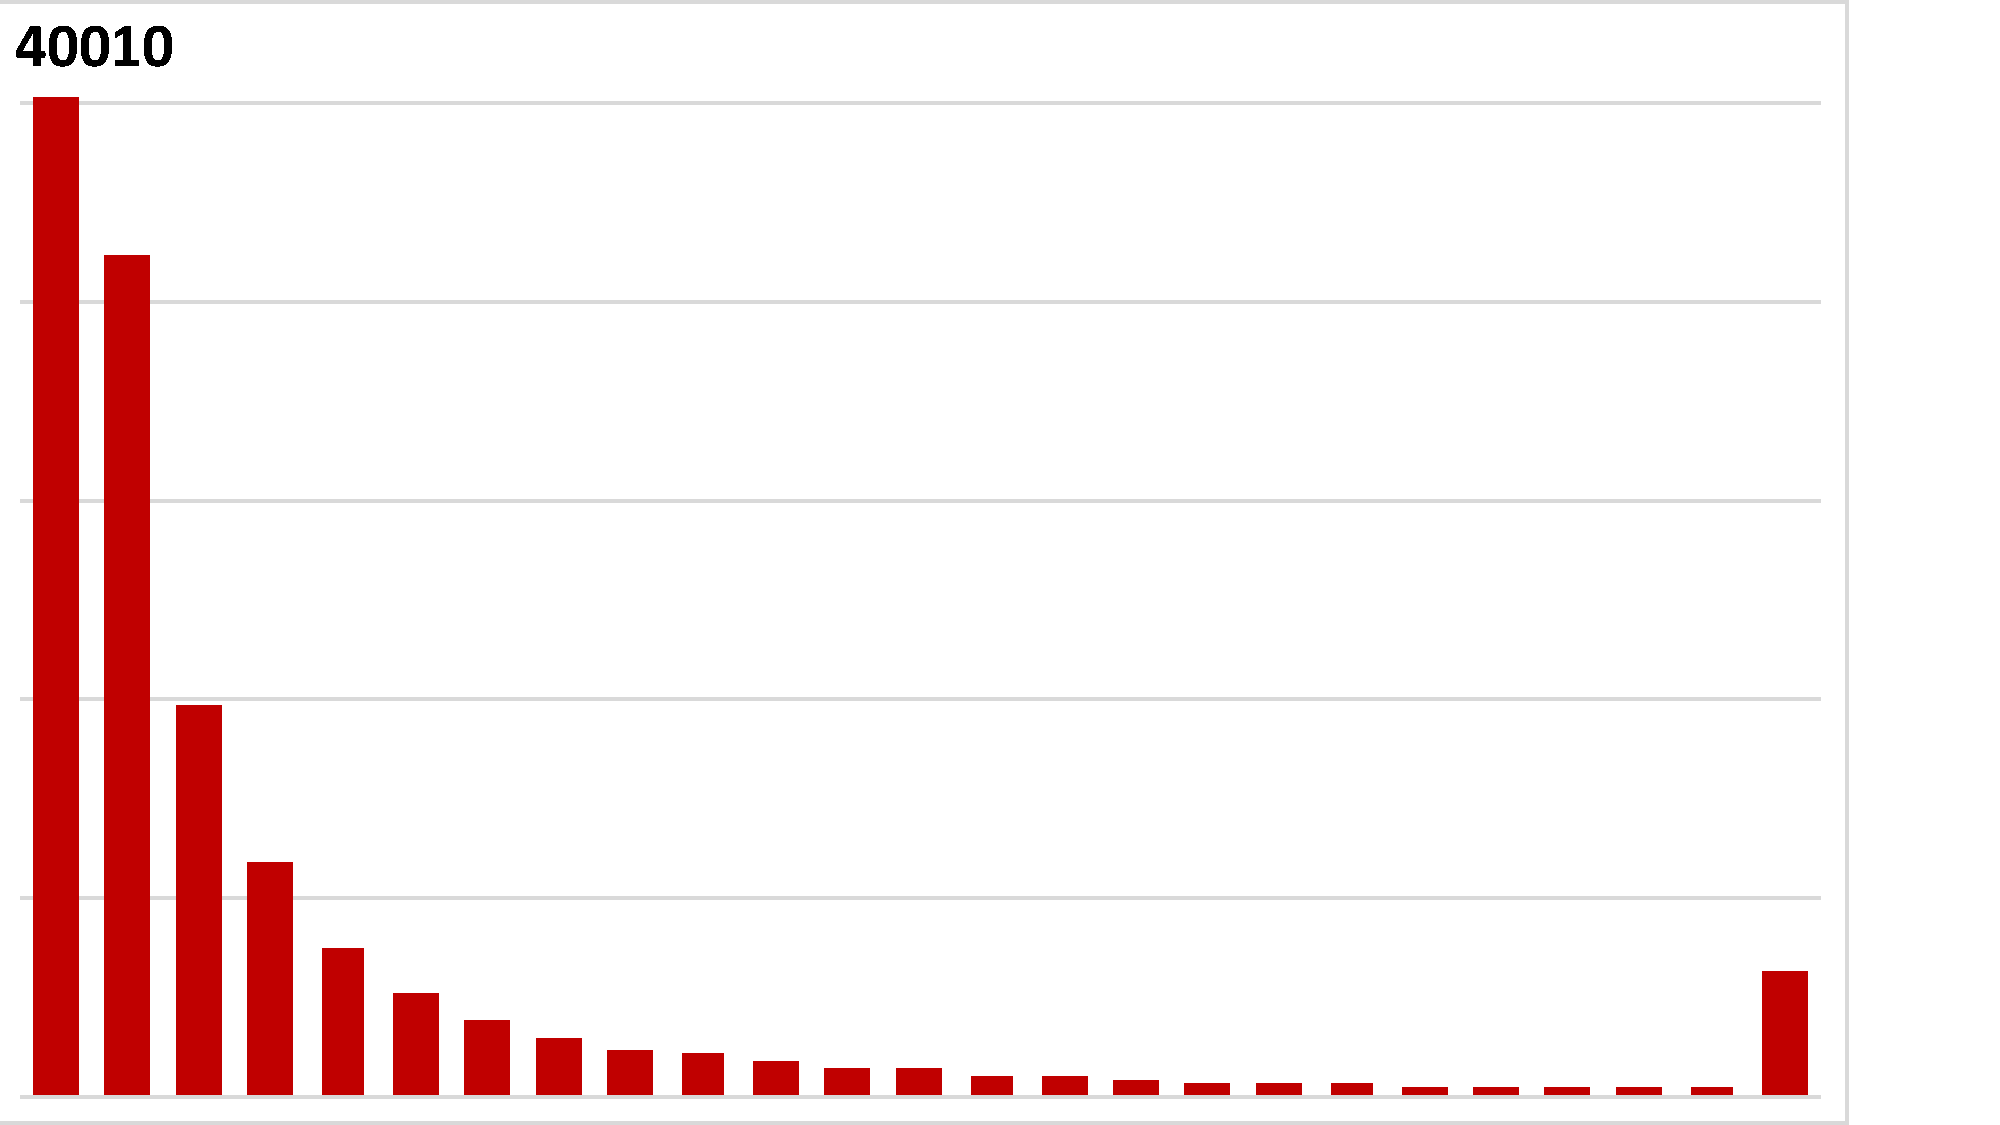
\includegraphics[width=0.9\linewidth, trim={0cm 0cm 2.5cm 0cm}, clip]{results/cloverleaf3d/lag_5/Lag5_Max.pdf}
\vspace{-2mm}
\caption{Lag 40 1:27 Max$_{L2}$}
\end{subfigure}
\begin{subfigure}{0.195\textwidth}
\centering
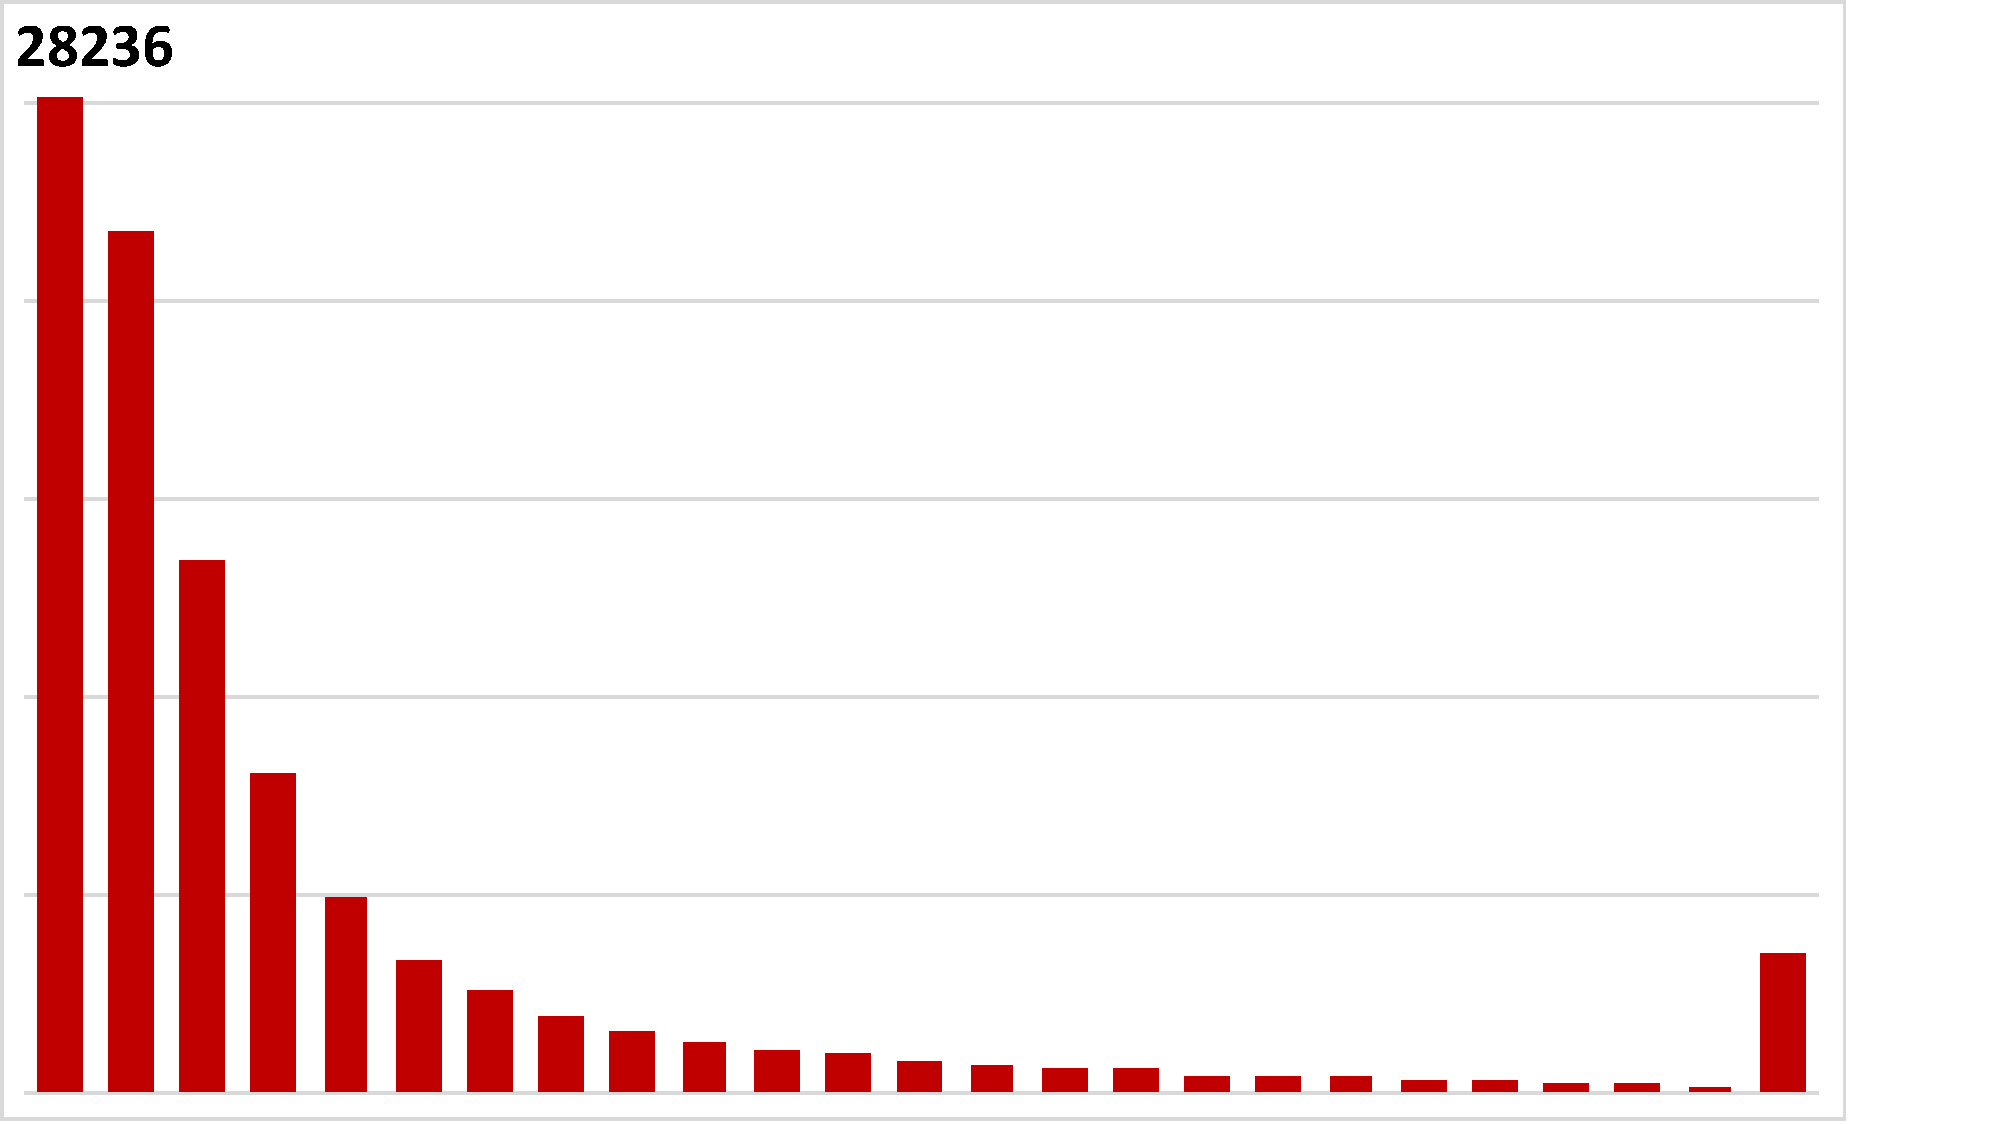
\includegraphics[width=0.9\linewidth, trim={0cm 0cm 2.5cm 0cm}, clip]{results/cloverleaf3d/lag_6/Lag6_Max.pdf}
\vspace{-2mm}
\caption{Lag 40 1:64 Max$_{L2}$}
\end{subfigure}
%\begin{subfigure}{0.24\textwidth}
%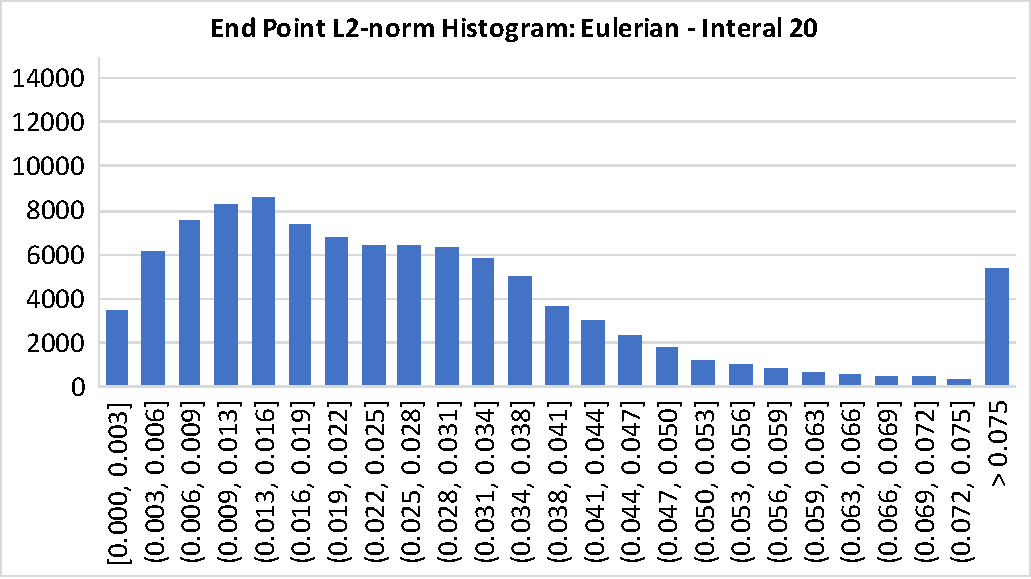
\includegraphics[width=0.9\linewidth]{results/cloverleaf3d/eul_1/Eul1_EndPt.pdf}
%\caption{Eulerian 20 End Point}
%\end{subfigure}
%\hspace{1mm}
%\begin{subfigure}{0.21\textwidth}
%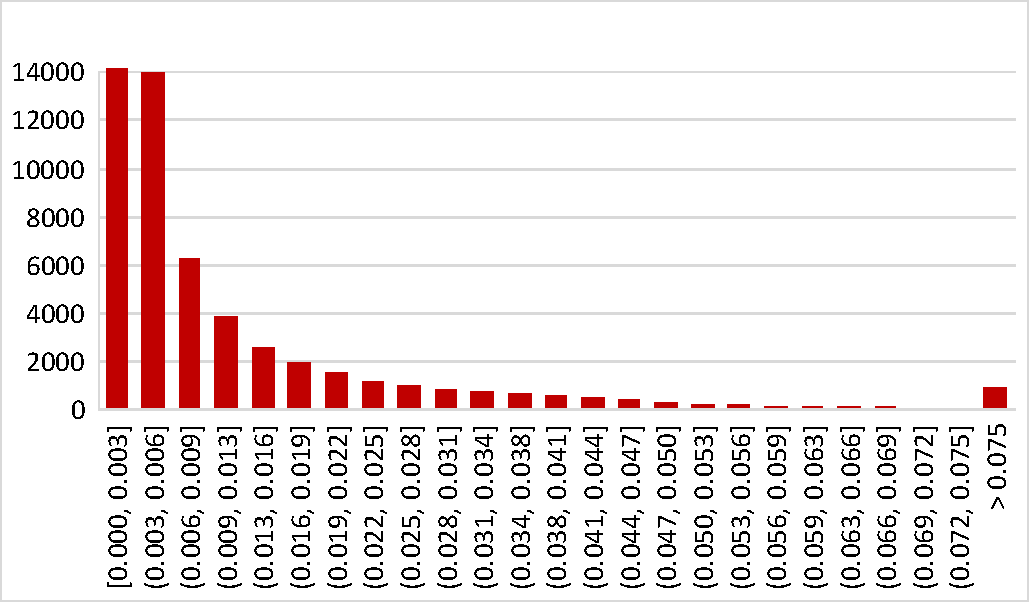
\includegraphics[width=1\linewidth]{results/cloverleaf3d/lag_4/Lag4_EndPt.pdf}
%\caption{Lagrangian 40 1:8 End Point}
%\end{subfigure}
%\hspace{1mm}
%\begin{subfigure}{0.21\textwidth}
%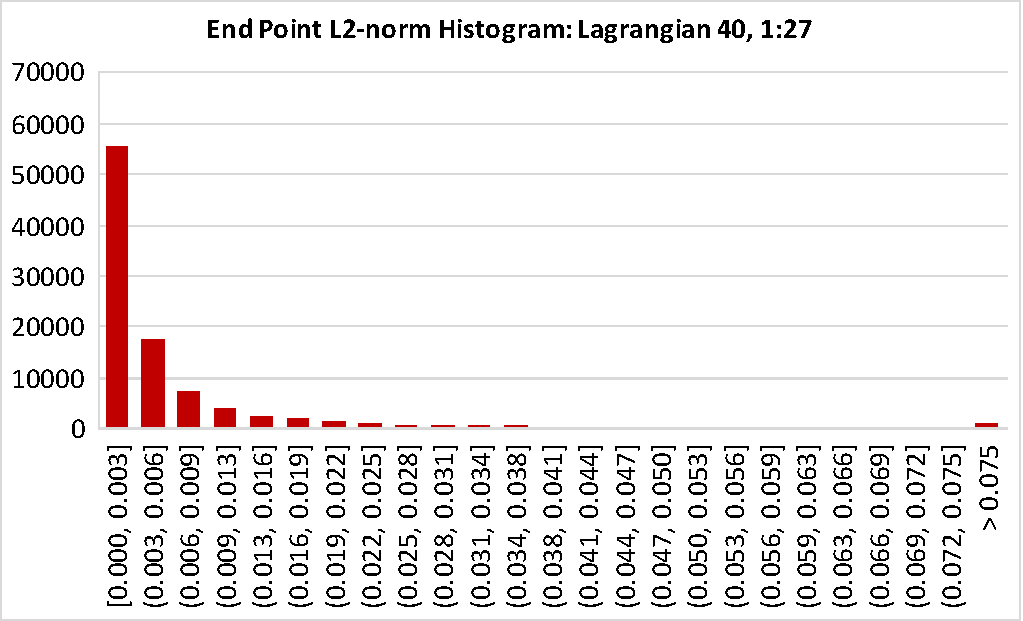
\includegraphics[width=1\linewidth]{results/cloverleaf3d/lag_5/Lag5_EndPt.pdf}
%\caption{Lagrangian 40 1:27 End Point}
%\end{subfigure}
%\hspace{1mm}
%\begin{subfigure}{0.21\textwidth}
%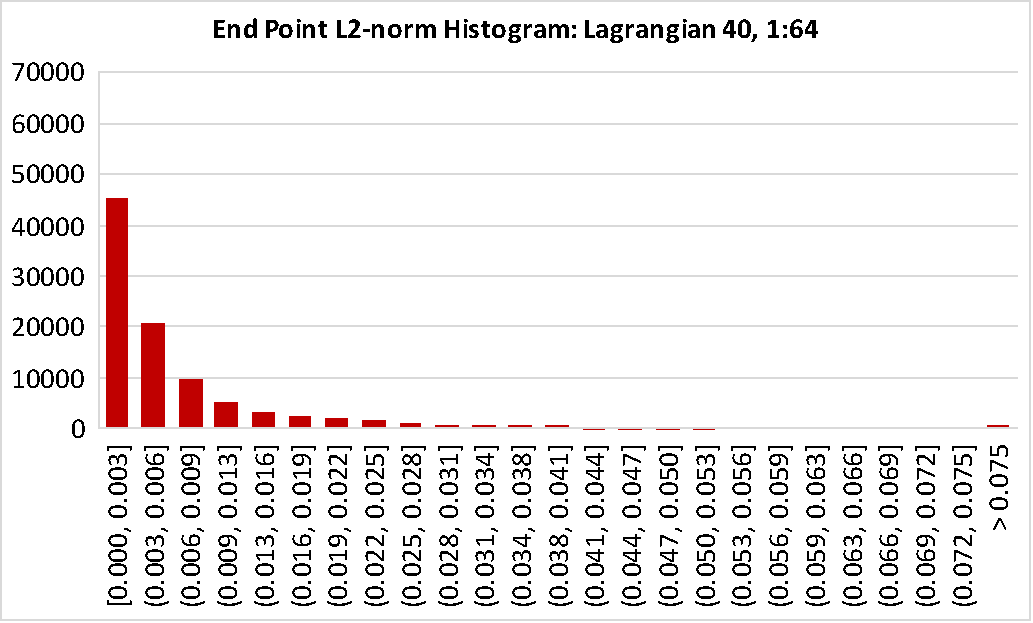
\includegraphics[width=1\linewidth]{results/cloverleaf3d/lag_6/Lag6_EndPt.pdf}
%\caption{Lagrangian 40 1:64 End Point}
%\end{subfigure}
\vspace{-3mm}
\caption{\textbf{Cloverleaf3D} experiment histograms for 100,000 test particle interpolation errors. Each plot has 25 bins, ranging from 0 to $>$0.05, with bar height encoding number of particles. Horizontal grid lines mark increments of 5,000.} 
\label{fig:clover_histograms}
\vspace{-6mm}
\end{figure*}

